It is difficult to apply traditional $K$NN query pruning strategies applicable for $K$D-Trees, to LISA model as it doesn't maintain a tree like structure with all nodes and
entries based on MBRs (minimum bounding rectangle) and parent-children relationships. %Shard boundaries are learned per mapped interval and no data structure is maintained to refer to shards in adjacent mapped intervals. 
The key idea in LISA paper $K$NN query implementation is to convert it into a range query by estimating an appropriate query range. LISA paper suggests a learning model to learn an appropriate distance bound from underlying training data for every query point and specific value of K. However, we have used empirically estimates to learn this distance bound for different values of $K$. This distance bound is used to convert the $K$NN query to range query.The query range is augmented if less than K neighbors are found in a range query. 

Consider a query point $q_{knn}=(x_{0},x_{1})$, let $x^{'} \in V$ be the $K$th nearest key to $x$ in database at a distance value $\delta = \| x^{'}-q_{knn}\|_{2} $. Lets define $ \mathcal{Q}(q_{knn},\delta) \triangleq [x_{0}-\delta, x_{0}+\delta) \times[x_{1}-\delta, x_{1}+\delta)$ and $\mathcal{B}(q_{knn}, \delta)  \triangleq \{p \in V \mid \| q_{knn}-p\|_{2} \leq \delta \} $. We can create a query rectangle $qr =  \mathcal{Q}(q_{knn}, \delta + \epsilon)$ where $\epsilon \rightarrow 0$. As shown in Fig. \ref{fig:KNN_Query_Lisa}, K nearest keys to $q_{knn}$ are all in $\mathcal{B}(q_{knn}, \delta)$ and thus in $\mathcal{Q}$. $K$NN query can be solved using the range query if we can estimate an appropriate distance bound $\delta$ for every query point.

\begin{figure*}[t]
    \centering
    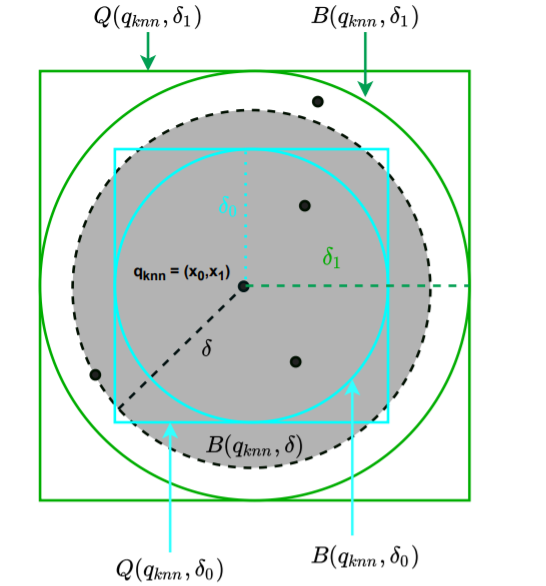
\includegraphics[width=0.7\textwidth]{graphs/KNN_Query_Lisa.png}
    \caption{KNN Query Implementation in Lisa(K=3)\\
    1)$q_{knn}$ represents the query point, $ \mathcal{Q}(x,\delta) \triangleq [x_{0}-\delta, x_{0}+\delta) \times[x_{1}-\delta, x_{1}+\delta)$, represents query rectangle and $ \mathcal{B}(x, \delta)$ represents the key space at distance $\delta$ containing K nearest keys.\\
    2)KNN query can be solved by range query if we can estimate an appropriate distance bound $\delta$ for every query point\\
    }
    \label{fig:KNN_Query_Lisa}
\end{figure*}
In our experiments, we find the $\delta$ empirically. We try with different values of $\delta$ and choose the one for which we get the best results. 